%%%%%%%%%%%%%%%%%%%%%%%%%%%%%%%%%%%%%%%%%%%%%%%%%%%%%%%%%%%%%%%%%%%%%%%%%%%%%%%%
%2345678901234567890123456789012345678901234567890123456789012345678901234567890
%        1         2         3         4         5         6         7         8

\documentclass[letterpaper, 10 pt, conference]{ieeeconf}  % Comment this line out if you need a4paper
\usepackage{graphicx}
\usepackage{url}
\usepackage{hyperref}
\usepackage{footnote}
\usepackage{caption}
\usepackage{amsmath}
\usepackage{amssymb}
\usepackage{siunitx}
\usepackage{soul, xcolor}

\newcommand{\tr}[1]{\textcolor{red}{#1}}
\setstcolor{red}

%German
% \usepackage{textcomp}
% \usepackage[T1]{fontenc}
% \usepackage[utf8]{inputenc} 

%\documentclass[a4paper, 10pt, conference]{ieeeconf}      % Use this line for a4 paper

\IEEEoverridecommandlockouts                              % This command is only needed if 
                                                          % you want to use the \thanks command

\overrideIEEEmargins                                      % Needed to meet printer requirements.

% See the \addtolength command later in the file to balance the column lengths
% on the last page of the document

% The following packages can be found on http:\\www.ctan.org
%\usepackage{graphics} % for pdf, bitmapped graphics files
%\usepackage{epsfig} % for postscript graphics files
%\usepackage{mathptmx} % assumes new font selection scheme installed
%\usepackage{times} % assumes new font selection scheme installed
%\usepackage{amsmath} % assumes amsmath package installed
%\usepackage{amssymb}  % assumes amsmath package installed

\title{\LARGE \bf
Object Detection with YOLO Algorithm}


\author{Piotr Mazurek}


\begin{document}



\maketitle
\thispagestyle{empty}
\pagestyle{empty}


%%%%%%%%%%%%%%%%%%%%%%%%%%%%%%%%%%%%%%%%%%%%%%%%%%%%%%%%%%%%%%%%%%%%%%%%%%%%%%%%
\begin{abstract}

This document is summary of my presentation about Object Detection with the YOLO Algorithm delivered on 25 February 2019 at the Seminar: Artificial Intelligence - Autonomous Vehicles WS 18/19 at FU Berlin. The seminar was conducted by Prof. Daniel G{\"o}hring. This document assumes that the reader is familiar with basic Algebra and Deep Learning concepts.

\end{abstract}


%%%%%%%%%%%%%%%%%%%%%%%%%%%%%%%%%%%%%%%%%%%%%%%%%%%%%%%%%%%%%%%%%%%%%%%%%%%%%%%%
\section{INTRODUCTION}

The YOLO Algorithm was introduced in 2015 by Joseph Redmon\footnote{University of Washington pjreddie@cs.washington.edu}, Santosh Divvala\footnote{Allen Institute for Artificial Intelligence santoshd@allenai.org}, Ross Girshick\footnote{Microsoft Research rbg@microsoft.com} and Ali Farhadi\footnote{University of Washington ali@cs.washington.edu}. The abbreviation YOLO stands for You Only Look Once and it explains the main concept of the algorithm. Currently YOLO is a state of the art algorithm for Object Detection problems. Since 2015, the authors have presented 2 improvements to the original YOLO paper: "YOLO9000: Better, Faster, Stronger" and "YOLOv3: An Incremental Improvement" They have described both as only minor changes to the original idea.

\section{WHY WE NEED OBJECT DETECTION FOR SELF-DRIVING CARS}
\begin{figure}[ht]
	\centering
    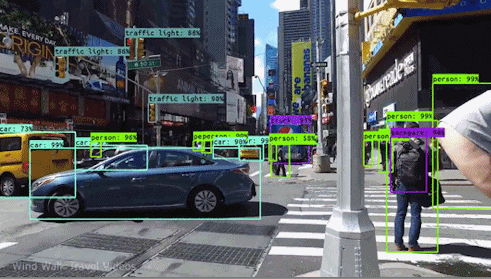
\includegraphics[width=0.45\textwidth]{Pictures/self_drive_see.png}
	\caption{How self-driving cars see the world [16]}
\end{figure}

Self-driving cars are the future of public transportation systems. Currently most autonomous vehicles use Lidar to detect objects in their surroundings. However, this is an imperfect solution, as  Lidars are expensive and can suffer from accuracy issues in certain circumstances (e.g. very bright sunlight may cause errors). Using some additional data would be very helpful to avoid mistakes. This additional data could be vision (See Fig. 1) - the basic data source based on which we (humans) drive our cars.

\section{WHAT TYPES OF OBJECTS COULD BE DETECTED USING YOLO}
% \begin{figure}[h]
% \centering
% 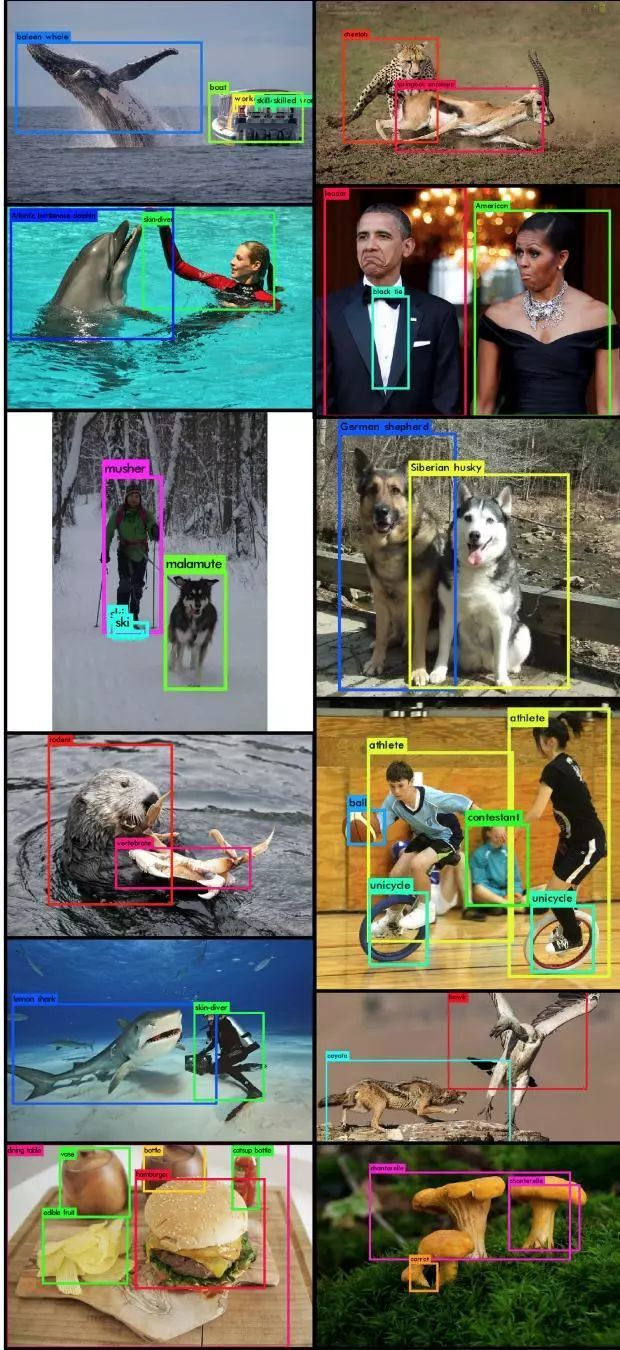
\includegraphics[scale=0.35]{Pictures/YOLO_Example_1.jpeg}
% \caption*{\newline How self driving car see the world}
% \end{figure}

In the earliest approaches to the Object Detection problem (Viola-Jones Algorithm, 2001 [5] and Histograms of Oriented Gradients, 2005 [6]) we were limited to the specified types of objects. We had to hand code n-features for each object and then provide it to a classifier. This approach worked for some objects like faces but didn't work for all objects. With YOLO we don't have that problem. It works for all types of objects, regardless of shape, size and color.

\section{INTUITIONS BEHIND CONVOLUTIONAL NEURAL NETWORKS}

The main concept behind YOLO is CNN (Convolutional neural network).This paragraph provides some intuition regarding how a CNN work and why we need it. 

\subsection{Why do we need CNN}

\begin{figure}[ht]
	\centering
    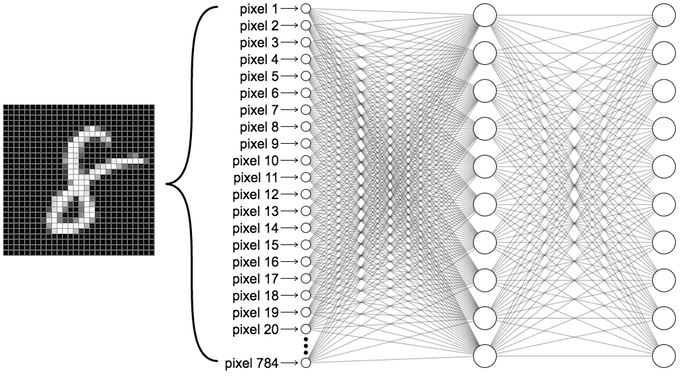
\includegraphics[width=0.5\textwidth]{Pictures/mnist_2layers.png}
	\caption{Neural Network for MNIST Dataset[18]}
\end{figure}

Simple computer vision problems like handwritten digit\st{s} recognition (e.g. MNIST Dataset), could be solved using traditional Neural Networks. We take an input data matrix of size $m \times  n$, convert it into an $(m*n) \times 1 $ vector, then we multiply it by NN weights, we add bias, we apply some non linear function (e.g. sigmoid $\sigma$) and we end up with the first layer of the NN. Then we do the same until we reach the last NN layer, which represents the NN prediction. For a 1 hidden layer NN it will look like that: 

$z_1 = (a_0 \times w_1) + b_1 $

$a_1 = \sigma(z_1) $

$z_2 = (a_1 \times w_2 ) + b_2 $

$a_2 = \sigma(z_2) $
\medskip \\
Where $a_0$ is input vector, $z_1$ is first hidden layer before applying a non-linear function activation, $a_1$ is first hidden layer after applying a non-linear function activation, $w_1$ is matrix of weights between $a_0$ and $a_1$, $b_1$ is bias we add to first hidden layer, analogously for $z_2$, $a_2$, $b_2$

We can solve the MNIST problem using traditional NN because it contains relatively small amount of features. Let us assume that the first layer contains 1000 Nodes. In that case for first layer we will have to train $785000$ features. (Fig. 2)

$(28 \times 28)_{image} \times 1000_{hidden \:layer \: nodes} + 1000_{bias} = \\ 784 \times 1000 + 1000 = 785 \: 000$ parameters

\vspace{5mm} %5mm vertical space

In the case of modern computers, it is feasible to store and optimize that amount of parameters, but what if instead of $28 \times 28$ gray picture we have $1000 \times 1000$ RGB picture?

\vspace{5mm} %5mm vertical space

$(1000 \times 1000)_{image} \times 3_{RGB \: channels} \times 1000_{hidden  \: nodes} = 3 \: 000 \: 000 \:000$ parameters

\vspace{5mm} %5mm vertical space

Such large number of parameters causes problems such as:

\begin{itemize}

\item It's very hard to store 3 billion parameters in memory, most of modern GPUs don't have enough memory

\item Optimizing 3 billion parameters is computationally expensive, training would take a lot o time

\item Overfitting, when we have too many parameters it is really hard to find "global optimum", our model will work better for data that it has been used for training then for new data (which is an unfortunate situation) 

\end{itemize}

So, what should we do instead if we want to work on real world pictures? We will come back to this problem later, because to solve it  we need to introduce concept of Edge Detection

\subsection{Edge detection}

One of the oldest way of solving computer vision problems is edge detection. Edge detection algorithm is performed using a matrix called a mask and an operation called convolution. The general expression of a convolution is:
\begin{equation}
    g(x, y)=(\omega * f)(x, y)=\sum_{s=-a}^{a} \sum_{t=-b}^{b} \omega(s, t) f(x-s, y-t)
\end{equation}

Where $g(x,y)$ is the filtered image, $f(x,y)$ is the original image, $\omega$ is the filter kernel. Every element of the filter kernel is considered by $-a \leqslant s \leqslant a$ and $-b \leqslant t \leqslant b$ [8]

   \begin{figure}[!ht]
      \centering
      \framebox{\parbox{3in}{$
\begin{bmatrix}
    0 & 0 & 0 & 10 & 10 & 10\\
    0 & 0 & 0 & 10 & 10 & 10\\
    0 & 0 & 0 & 10 & 10 & 10\\
    0 & 0 & 0 & 10 & 10 & 10\\
    0 & 0 & 0 & 10 & 10 & 10\\
    0 & 0 & 0 & 10 & 10 & 10\\
\end{bmatrix}_{img} * \begin{bmatrix}
    -1 & 0 & 1\\
    -1 & 0 & 1\\
    -1 & 0 & 1\\
\end{bmatrix}_{mask} = $ 
\vspace{5mm} %5mm vertical space

$\begin{bmatrix}
    0 & 30 & 30 & 0\\
    0 & 30 & 30 & 0\\
    0 & 30 & 30 & 0\\
\end{bmatrix}_{detected \: edge}
$
}}
      %\includegraphics[scale=1.0]{figurefile}
      \caption{Example convolution operation [15]}
      \label{figurelabel}
   \end{figure}
\vspace{5mm} %5mm vertical space   

Example cells from detected edge matrix (Fig. 3)

E.g: $f(1,2) = (0 \times -1) + (0 \times -1) + (0 \times -1) + (10 \times 0) + (10 \times 0) + (10 \times 0) + (10 \times 1) + (10 \times 1) + (10 \times 1) = 0 + 0 + 0 + 0 +0 + 0 + 10 + 10 + 10 = 30$
\vspace{5mm} %5mm vertical space

E.g: $f(3,4) = (10 \times -1) + (10 \times -1) + (10 \times -1) + (10 \times 0) + (10 \times 0) + (10 \times 0) + (10 \times 1) + (10 \times 1) + (10 \times 1) = -10 -10 -10 + 0 +0 + 0 + 10 + 10 + 10 = 0$

\subsection{Masks examples}

In traditional computer vision algorithms filter values were hand-engineered. The most basic examples of  hand-engineered filters are: Sobel Filter or Haar Filter. They allow us to detect relatively simple image features (see Fig. 4 \& Fig. 5). 

   \begin{figure}[!ht]
      \centering
      \framebox{\parbox{3in}{
      $\begin{bmatrix}
    -1 & 0 & 1\\
    -2 & 0 & 2\\
    -1 & 0 & 1\\
    \end{bmatrix}_{0} $       $\begin{bmatrix} 
    0 & 1 & 2\\
    -1 & 0 & 1\\
    -2 & -1 & 0\\
    \end{bmatrix}_{45} $  $\begin{bmatrix}
    1 & 2 & 1\\
    0 & 0 & 0\\
    -1 & -2 & 1\\
    \end{bmatrix}_{90} $ 
    }}
      
      \caption{Example edge detection Sobel filter for angles: \ang{0}, \ang{45} and \ang{90}}
      \label{figurelabel}
   \end{figure}
   
   
      \begin{figure}[!ht]
      \centering
      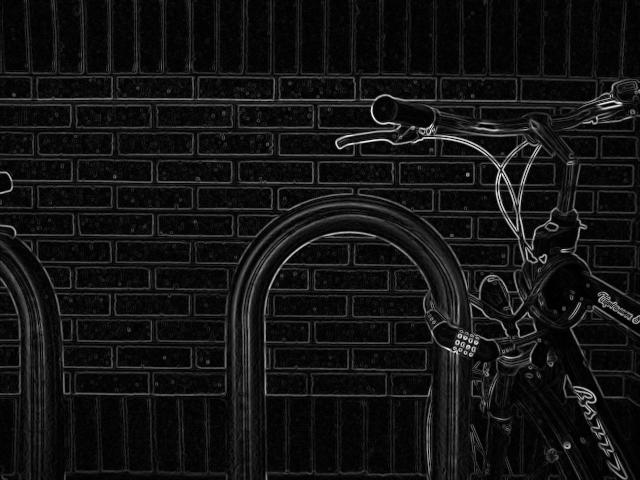
\includegraphics[scale=0.35]{Pictures/Bikesgraysobel.jpg}
      \caption{Detected edges after applying Sobel filter [17]}
      \label{figurelabel}
   \end{figure}



\subsection{What if we don't know filter values}

Using hand-engineered filters values we can detect horizontal or vertical edges quite good but what if we want to detect some more sophisticated features like cat edges? 

\begin{figure}[ht]
	\centering
    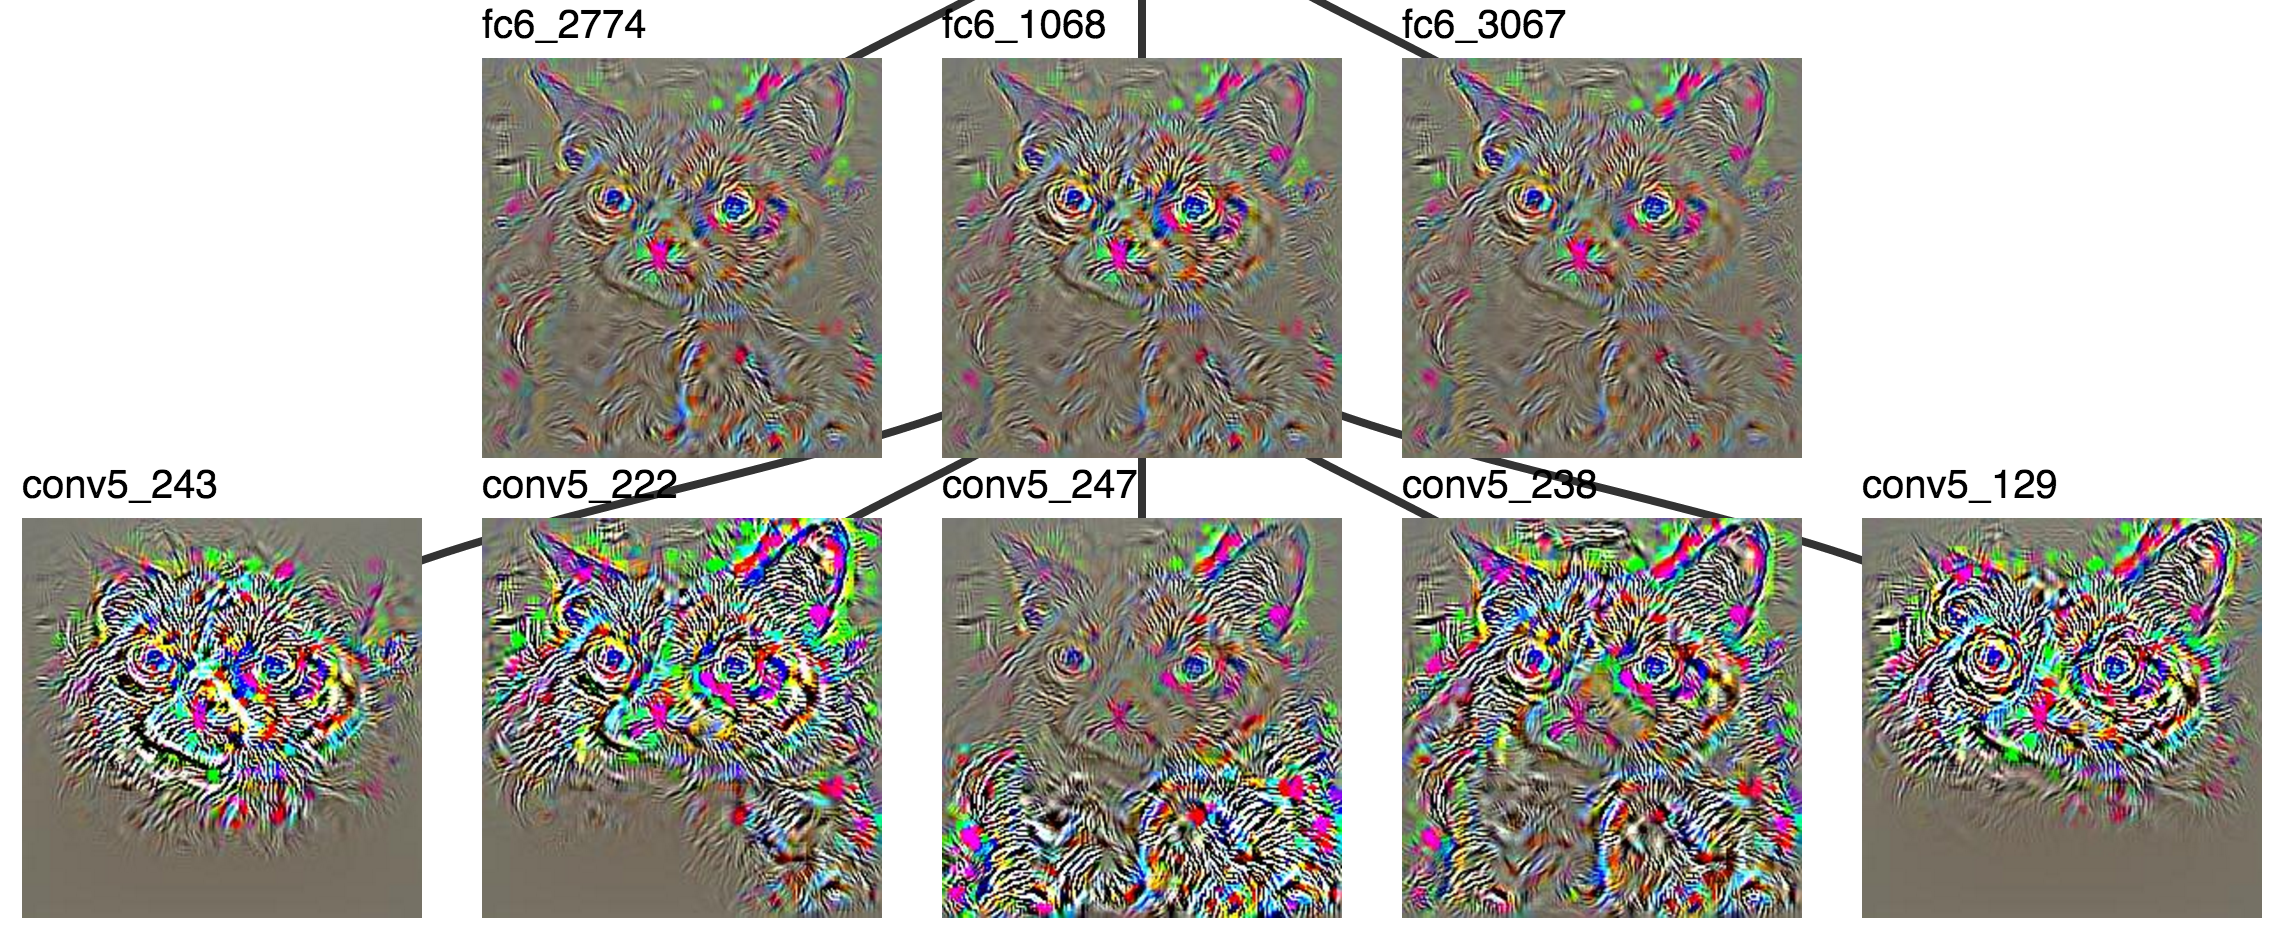
\includegraphics[width=0.5\textwidth]{Pictures/cat eatures.png}
	\caption{Cat features recognized by individual CNN layers [10]}
\end{figure}

This is where deep learning comes in: Instead of using hand-engineered filter values we can use a self-learning algorithm that finds the right values by itself (like in Fig. 6).

   \begin{figure}[!ht]
      \centering
      \framebox{\parbox{3in}{$
\begin{bmatrix}
    0 & 0 & 0 & 10 & 10 & 10\\
    0 & 0 & 0 & 10 & 10 & 10\\
    0 & 0 & 0 & 10 & 10 & 10\\
    0 & 0 & 0 & 10 & 10 & 10\\
    0 & 0 & 0 & 10 & 10 & 10\\
    0 & 0 & 0 & 10 & 10 & 10\\
\end{bmatrix}_{img} * \begin{bmatrix}
    w_1 & w_2 & w_3\\
    w_4 & w_5 & w_6\\
    w_7 & w_8 & w_9\\
\end{bmatrix}_{mask}$ 
}}
      \caption{Instead using hand-engineered filter values we use learned values [15]}
      \label{figurelabel}
   \end{figure}


What is interesting at this point is the fact that regardless of the image size, we have same number of parameters to train. No matter if our image is $20 \times 20$ pixels or $1000 \times 1000$ we need to train the same number of parameters - the number of values in filter mask (See Fig. 7). It is one of main reasons why CNNs are so popular in real life computer vision problems.

\section{ARCHITECTURE OF CONVOLUTIONAL NEURAL NETWORK}
Quick reminder about basics of CNN and introduction of naming convention used further in this paper.

\subsection{Convolution layer}
The role of the convolution layer is to apply the convolution operation to the image by using the filter mask. Values from filter mask are parameters which we are training (See Fig. 8). 

\begin{figure}[ht]
	\centering
    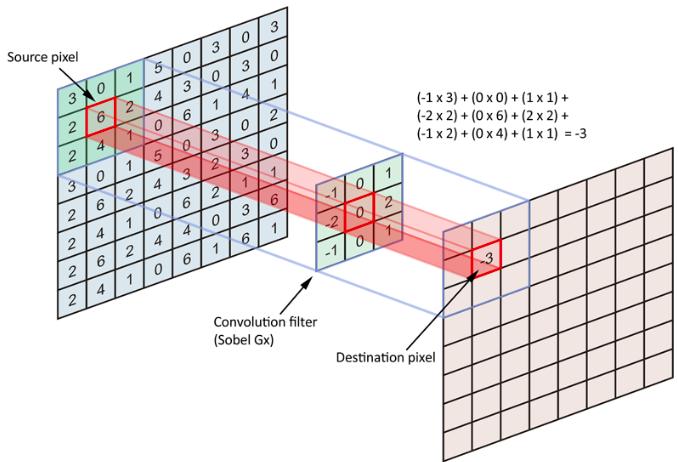
\includegraphics[width=0.4\textwidth]{Pictures/ConvolutionLayer.png}
	\caption{Convolution operation example [11]}
\end{figure}

\subsection{Convolution operation on volume}

The previous examples contained only one channel, but in real life we usually have more. E.g. colorful RGB Image contains 3 channels (Red, Green, Blue). In that case each filter need to have 3 "sub filters", one for each channel. We apply convolution operation to each channel and then sum up the result (See Fig. 9).  

\begin{figure}[h]
	\centering
    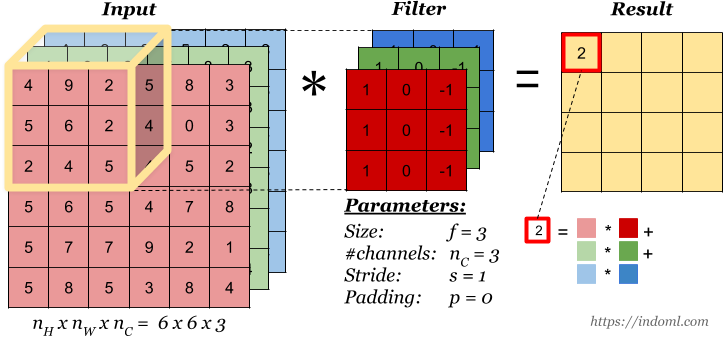
\includegraphics[width=0.4\textwidth]{Pictures/convolution-operation-on-volume5.png}
	\caption{Convolution operation on volume example [12]}
\end{figure}

% 

\subsection{Multiple filters}

To detect multiple types of features in previous layer we should use multiple filters. E.g. one filter will detect vertical edges and one will detect horizontal. In this paper we consider the last number of output as number of filters used in convolution operation (See Fig. 10).

\begin{figure}[!ht]
	\centering
    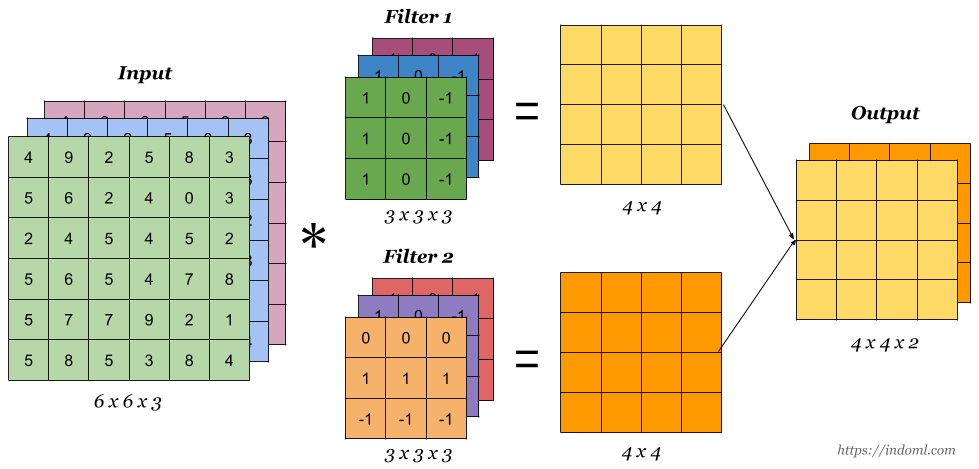
\includegraphics[width=0.5\textwidth]{Pictures/convolution-with-multiple-filters2.png}
	\caption{Example of using 2 filters [12]}
\end{figure}

\subsection{Padding}

To avoid under representation of edge pixels it is worth to add extra one layer of extra pixels around original image (See Fig. 11).

\begin{figure}[!ht]
	\centering
    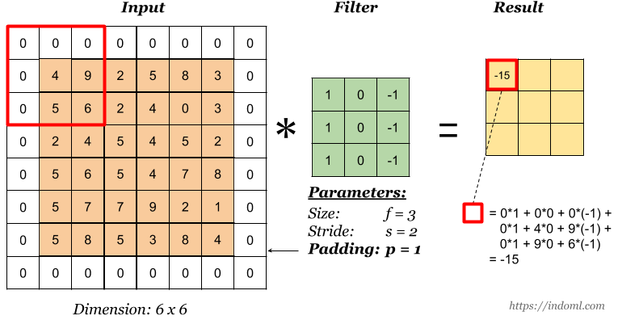
\includegraphics[width=0.5\textwidth]{Pictures/padding.png}
	\caption{Example of 1 pixel padding [12]}
\end{figure}

\subsection{Stride}

Stride determines the number of cells that the filter moves in the input to calculate cell in output (See Fig. 12).

\begin{figure}[!ht]
	\centering
    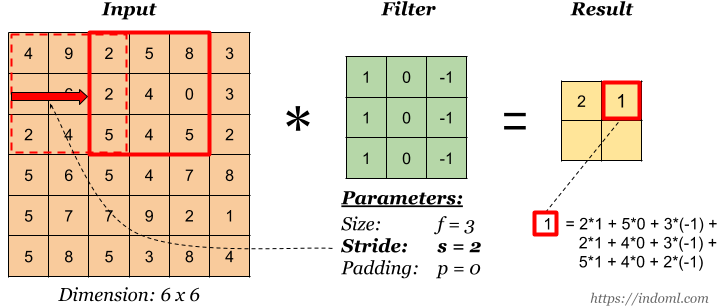
\includegraphics[width=0.5\textwidth]{Pictures/stride.png}
	\caption{Example of stride = 2 [12]}
\end{figure}

\subsection{Pooling layer}

Second type of layers used in CNNs is Pooling Layer. There are two types of Pooling Layers: Avg. Pooling and Max Pooling. Pooling layer is mainly used to reduce size of outputs (See Fig. 13)

\begin{figure}[!ht]
	\centering
    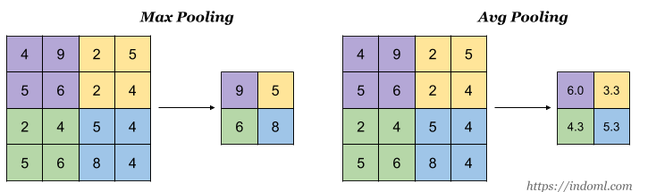
\includegraphics[width=0.5\textwidth]{Pictures/pooling-layer3.png}
	\caption{Example of pooling layer [12]}
\end{figure}


\subsection{Fully Connected layer}

FC layer is a layer where every neuron from previous layer is connected to every neuron in next layer. It is in principle the same as the traditional Neural Network.

\subsection{Example CNN architecture}
Traditionally CNNs have been used to solve image recognition problems. The last FC layer was a prediction layer. On the image below (Fig. 14) we can see LeNet-5. LeNet-5 was able to achieve error rate below 1\% on the MNIST data set. 

\begin{figure}[!ht]
	\centering
    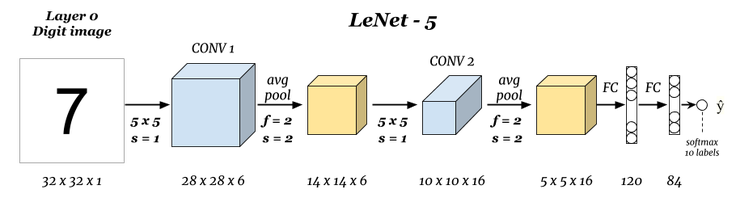
\includegraphics[width=0.5\textwidth]{Pictures/lenet-52.png}
	\caption{Example CNN - LeNet 5 from 1998 [12]}
\end{figure}


\subsection{Convert FC layer to Convolutional layer}
Interesting "trick" is we can implement FC layer by using convolution filters. Amount of filters should correspond the amount of Nodes that we wanted to achieve by applying FC layer.  Mathematically it is exactly the same, we have same amount of features to train but we will spot later that this "trick" will be very useful for YOLO algorithm (See Fig. 15). 

\begin{figure}[!ht]
	\centering
    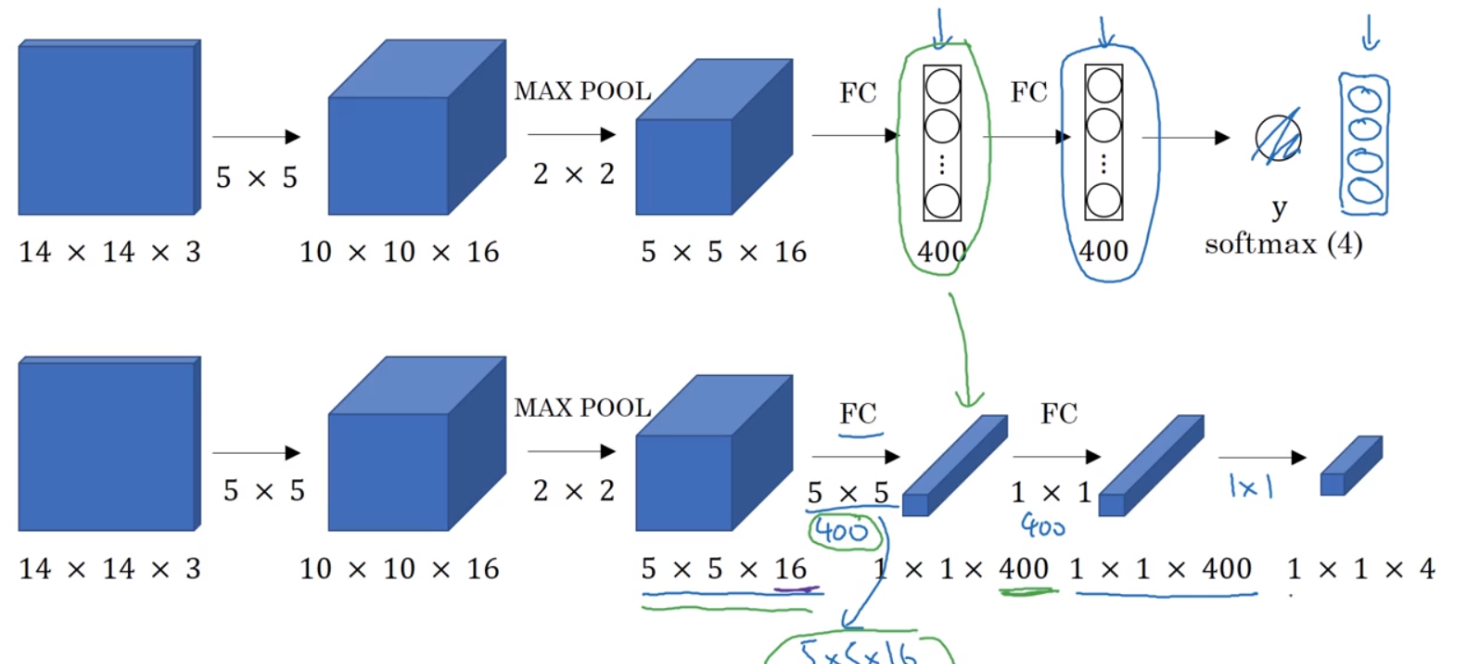
\includegraphics[width=0.5\textwidth]{Pictures/FC_to_conv.png}
	\caption{Example of FC layer converted into convolution[15]}
\end{figure}

\section{OBJECT LOCALIZATION}

Object Localization is a simplified version of object detection problem, where image contains only one big object of some class. The goal of NN is to predict if image contains any object and if so, to predict central point coordinates, width and high. Very similar concept will be used further in this paper to describe how YOLO Algorithm works. For the purposes of this paper to avoid problems with size of an image, let's assume that the top left corner will be described as point $(0,0)$ and bottom right corner  will be described as point $(1,1)$ (Example outputs at Fig. 16)

\begin{figure}[!ht]
	\centering
      \framebox{\parbox{3.35in}{
          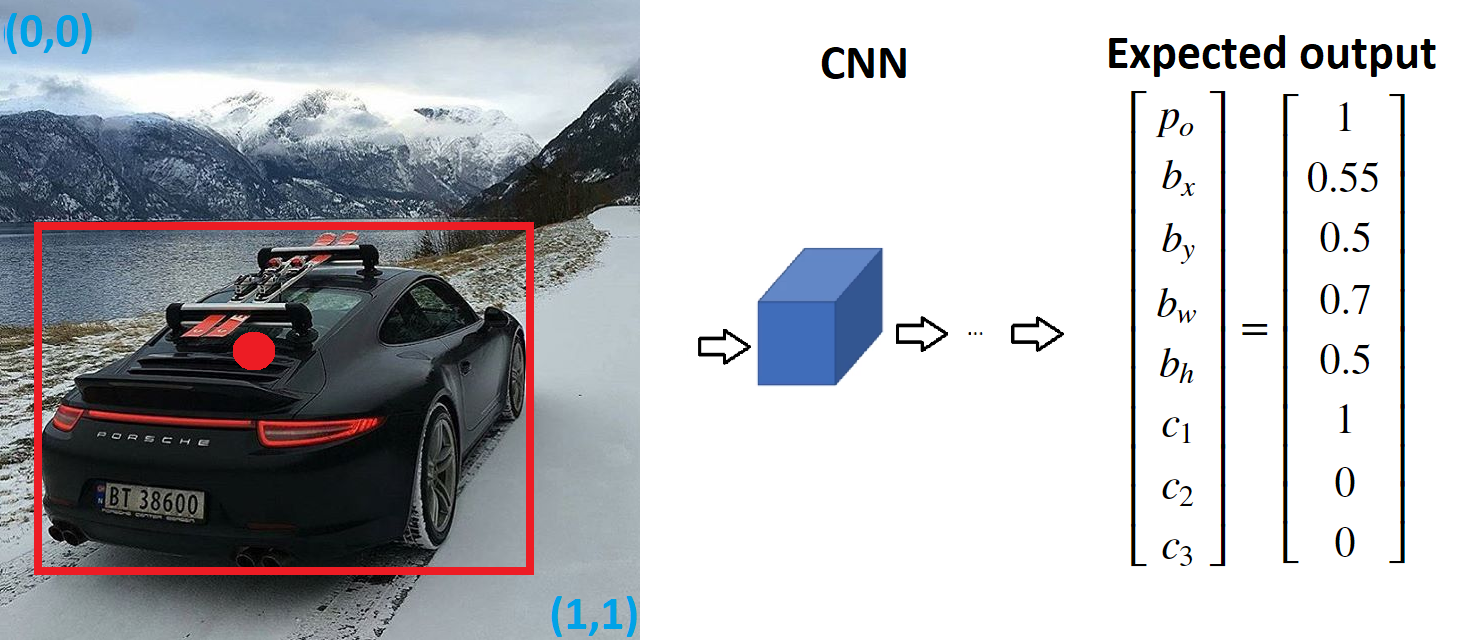
\includegraphics[width=0.45\textwidth]{Pictures/expected_output__object_localisation.png}
          
          \vspace{5mm} %5mm vertical space

          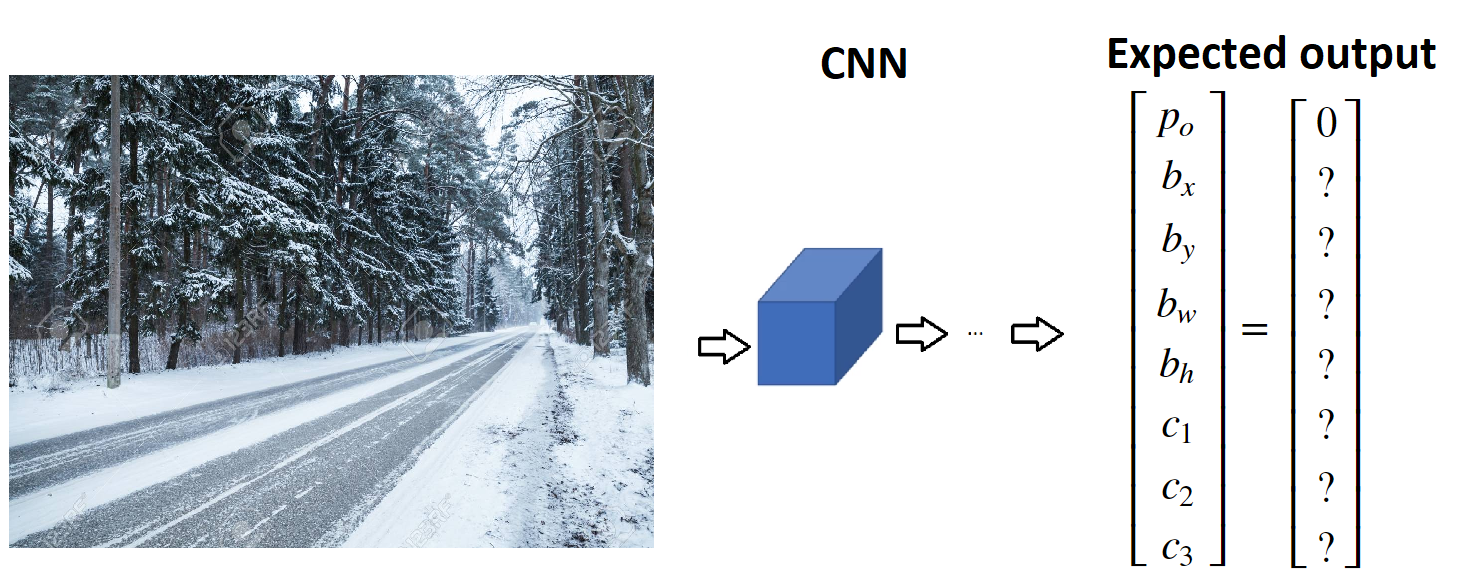
\includegraphics[width=0.45\textwidth]{Pictures/empty_expected_output__object_localisation.png}
         }}

	\caption{Example Object Localization Output}
\end{figure}

$?$ means that this element of vector doesn't matter so here could be anything

Loss function could be designed like that:

\begin{equation}
 L(\hat{y},y)=\left\{
  \begin{array}{@{}ll@{}}
    (\hat{y_1} - y_1)^2 + \dots + (\hat{y_n} - y_n)^2 & \text{if}\ y_1=0 \\
    (\hat{y_1} - y_1)^2 & \text{if}\ y_1=1
  \end{array}\right.
\end{equation} 

Where $y_1 = p_o, \: y_2 = b_x, \: y_3=b_y$ etc.

\section{SLIDING WINDOW}
If image contains more then one object we can no longer use Object Localization, so we need to find another way to detect objects. One of popular approaches is sliding window algorithm. It is very simple but provide good enough results. 

\subsection{How algorithm works}
Sliding window algorithm, as the name suggests is mainly about sliding a window. We take same part of an image, feed forward it through Neural Network (or any other classifier) and we have prediction if this part of an image contains object. 

\subsection{Why it is not perfect}
Sliding window approach is relatively simple but unfortunately it has a few disadvantages, such as:

\begin{itemize}

\item We know neither size nor shape of an object we are looking for

\item We need to feed forward thousands of images through classifier which is computationally expensive

\item We don't know which stride to choose, if we choose to small we will work many times on nearly same image, if we choose too big accuracy will be really poor


\end{itemize}

So how we can make it in a smarter way?


\section{CONVOLUTIONAL IMPLEMENTATION OF SLIDING WINDOW}
We can perform sliding window much faster and more efficient using its Convolution implementation. The idea of Convolutional implementation of sliding window was first introduced in Feb. 2014 by Sermanet\footnote{New York University sermanet@cs.nyu.edu},  Eigen\footnote{New York University deigen@cs.nyu.edu}, Zhang\footnote{New York University xiang@cs.nyu.edu}, Mathieu\footnote{New York University mathieu@cs.nyu.edu}, Fergus\footnote{New York University fergus@cs.nyu.edu}, LeCun\footnote{New York University yann@cs.nyu.edu}  in "OverFeat: Integrated Recognition, Localization and Detection using Convolutional Networks" paper. One year later it was used in the original YOLO paper. 

\subsection{How it works}
Using convolutions we can share a lots of computations. We apply convolution operation to an original image, and we "accumulate" knowledge about individual regions in cells of next layer. Then we apply next convolution we "accumulate accumulated" knowledge and so on and so forth. We end up having information about regions in a single cell of the last output. More on that in the original paper. (See Fig. 17) 

\begin{figure}[!ht]
	\centering
    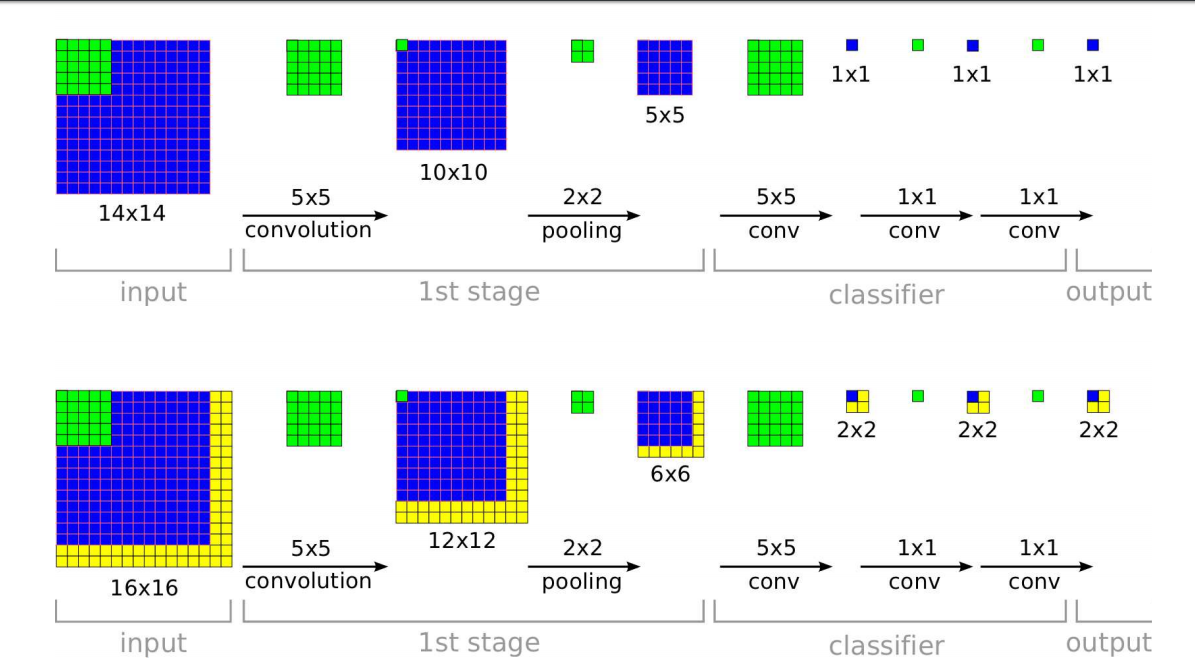
\includegraphics[width=0.5\textwidth]{Pictures/Convlutional_sliding_window.png}
	\caption{Example of Conv implementation of sliding window [13]}
\end{figure}

\section{YOU ONLY LOOK ONCE}
Finally we've reached YOLO - You Only Look Once. YOLO combines the ideas from convolution implementation of sliding window and object localization.
\begin{figure}[!ht]
	\centering
    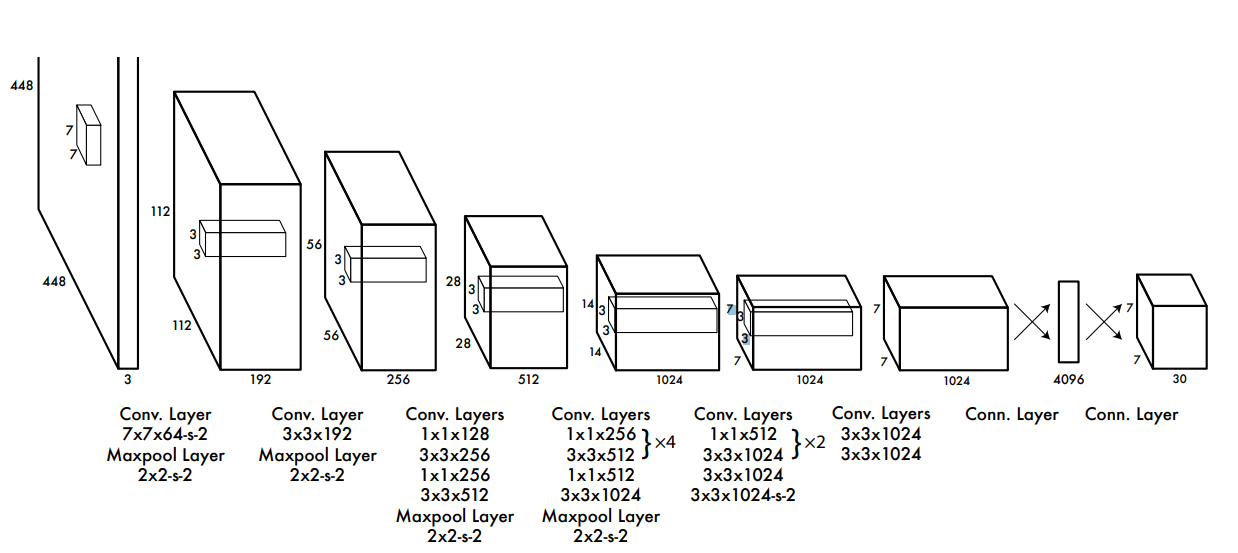
\includegraphics[width=0.5\textwidth]{Pictures/YOLO_architecture.png}
	\caption{Original YOLO Architecture [1]}
\end{figure}

\subsection{How it works}
In YOLO we apply convolution implementation of sliding window to the input image, we end up with image divided into some kind of grid cell. Each cell combines information about itself and surrounding cells. Each cell represents vector similar to the one that we know from object localization. It contains probability that cell contains central point of some object, the coordinates of that central point (to avoid problems with size we assume that top left corner of a each grid cell has coordinates $(0,0)$ and bottom right corner has coordinates $(1,1)$), object width and high (it might me be grater then one, because cell has knowledge also about cells surrounding it) and probabilities of classes(In Fig. 19 example output for a single cell). 

E.g. In the original YOLO architecture last output is $7 \times 7 \times 30$ (See Fig. 18) it means that we have 49 grid cells and each cell is vector of 30 elements which describe that grid cell. 

\begin{figure}[!ht]
	\centering
    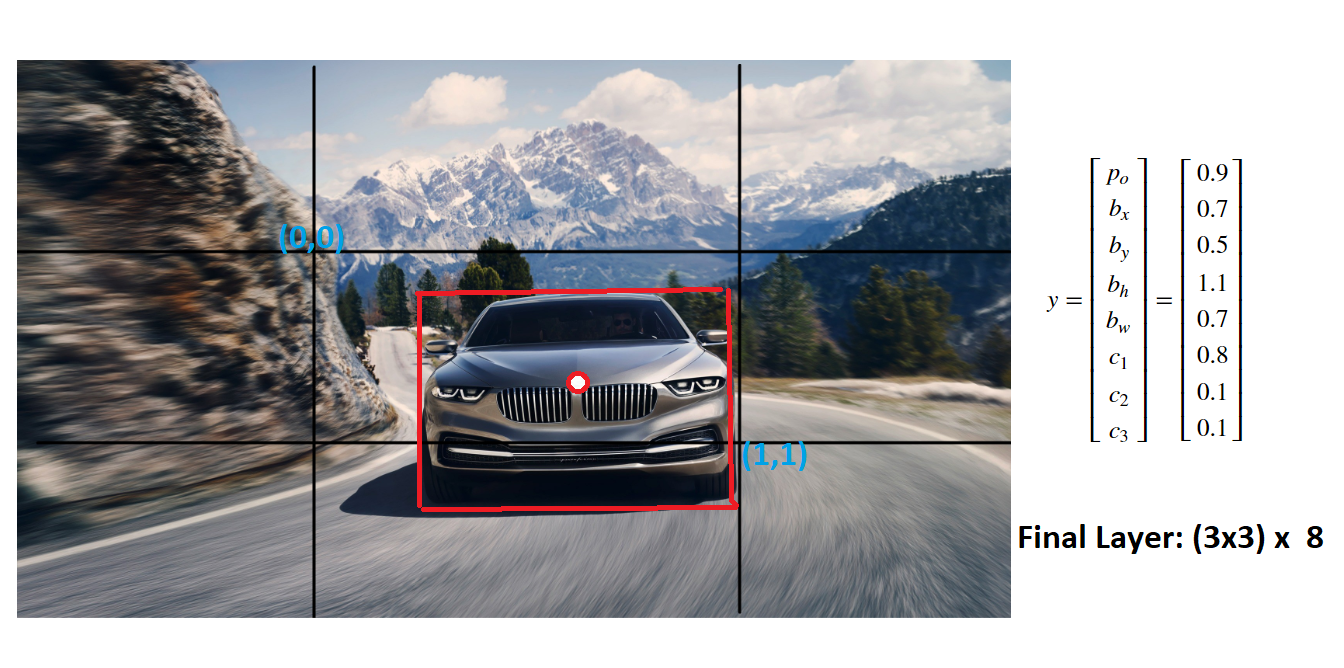
\includegraphics[width=0.5\textwidth]{Pictures/YOLOExampleOutput2.png}
	\caption{Example cell output for $ (3\times 3) \times 8$ output layer}
\end{figure}

After propagating our image through CNN we have prediction for every cell. To get a final predictions we need to perform 2 steps (See result of these 2 steps in Fig. 20)

\begin{itemize}

\item Remove all predictions where $p_o$ is smaller then some threshold value, so remove all predictions where probability that cell contains central point of an object is smaller then e.g 50\%.  

\item Using Non-max suppression get rid of rest useless predictions
\end{itemize}


\begin{figure}[!ht]
	\centering
    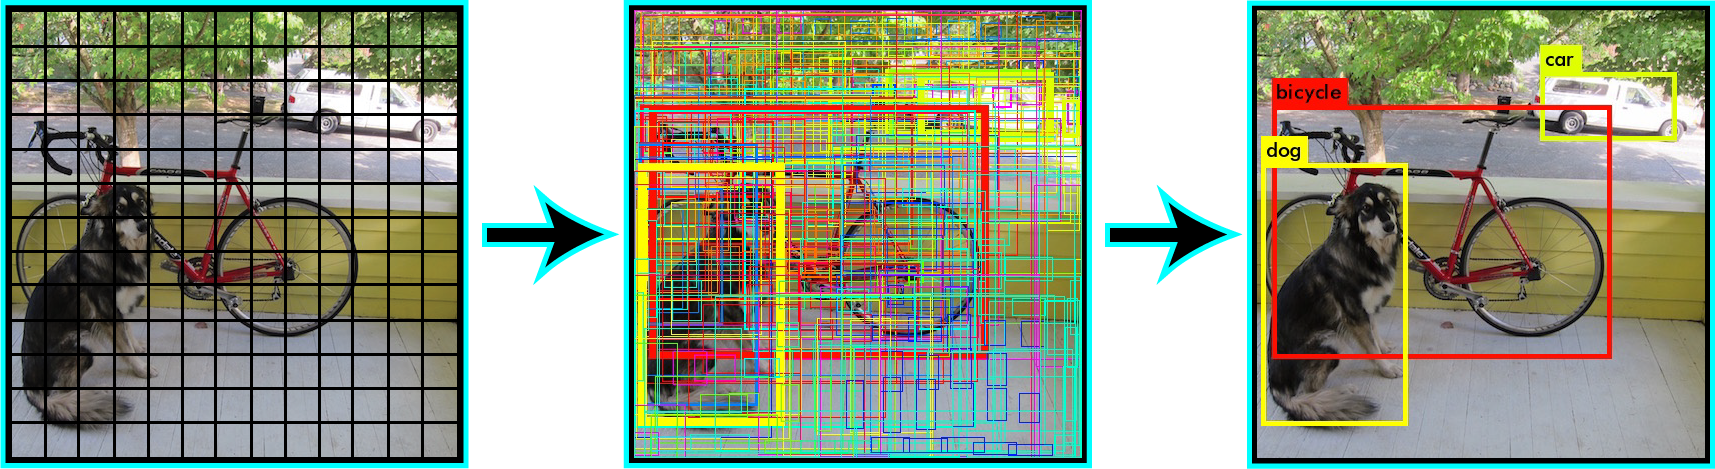
\includegraphics[width=0.5\textwidth]{Pictures/YOLO_grid_cell.png}
	\caption{Predictions for $(13 \times 13)$ grid cell after Non-max suppression [1]}
\end{figure}

\subsection{Non-max suppression}
When we have 2 predictions that intersect, we need to decide, should both predictions be kept, because they detect 2 objects or is it the same object and one of them should be removed. To solve that problem we need to introduce the idea of $IoU$

$IoU$ - Intersection over Union. As the name suggests is a fraction $\frac{Intersection \: surface \: area}{Union \: surface \: area}$

In Non-max suppression we compere surface of intersection with surface of union and when $IoU$ is bigger then some threshold value (e.g. 0.6, but it depends on implementation) we take only the detection with bigger $p_o$ - probability that this cell contains central point of an object. In case $IoU$ is smaller then some threshold value we keep both predictions. We perform Non-max suppression for all intersecting predictions. (Example result of algorithm in Fig. 21) 

\begin{figure}[!ht]
	\centering
    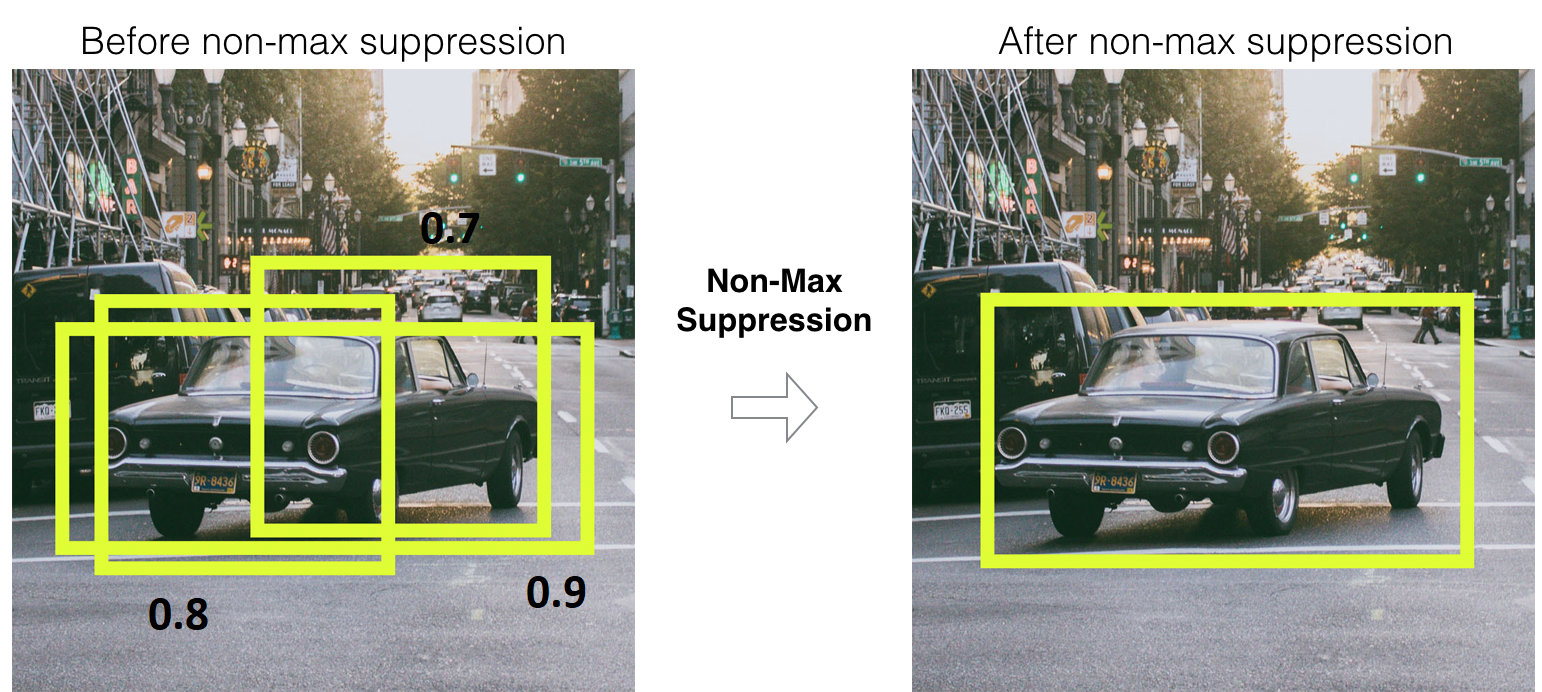
\includegraphics[width=0.5\textwidth]{Pictures/Non_max_supression.png}
	\caption{Example of Non-max suppression algorithm result [19]}
\end{figure}


\subsection{Anchor box}
The idea of anchor box was introduced in YOLO9000 paper. Concept is relatively simple. What happen when two objects of different shapes or different sizes has central point in the same cell? In that case in the original YOLO paper only one object could be detected. In improved version of algorithm the last layer of CNN (the one that divide image into grid cells) is "deeper", it contains multiple predictions not only one. 

The size of each grid cell will be (number of anchor boxes) $\times$ (size of original prediction). Thanks to that it is possible to detect multiple object in one grid cells.

In YOLO9000 authors used 5 anchor boxes and in YOLOv3 9. Instead of choosing anchors by hand, authors run k-means clustering on the training set bounding boxes to automatically find good anchors (Example output in Fig. 22). 


\begin{figure}[!ht]
	\centering
      \framebox{\parbox{3.35in}{
          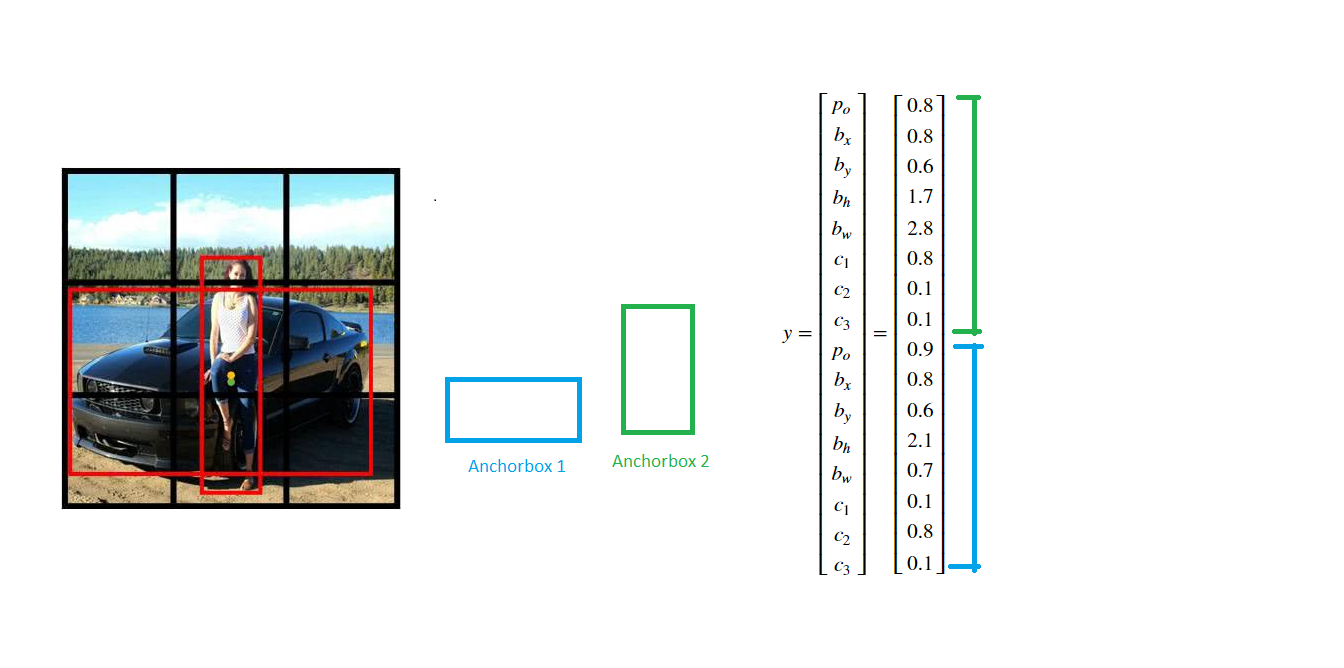
\includegraphics[width=0.65\textwidth]{Pictures/AnchorBoxesExample.png}
         }}

	\caption{Example output for CNN with 2 anchor boxes}
\end{figure}


\section{CONCLUSIONS}
YOLO is a real-time, universal object detection algorithm. It combines high performance with a  high accuracy (See Fig. 23), so it can be used to solve real-world problems. In future it can be used in self-driving cars to create safer future for all of us.

\begin{figure}[!ht]
	\centering
    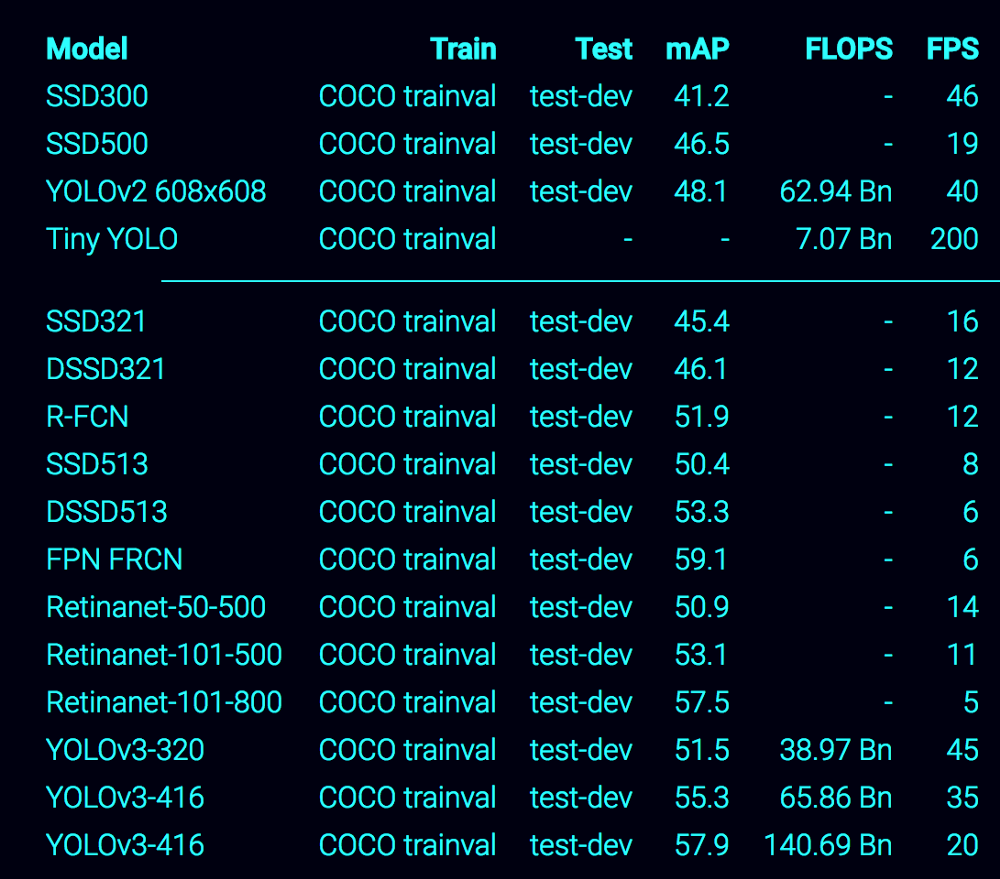
\includegraphics[width=0.5\textwidth]{Pictures/yolo_stats.png}
	\caption{Comparison of the best object detection algorithms [14]}
\end{figure}



\begin{thebibliography}{99}

\bibitem{c1} Original YOLO paper: \url{https://arxiv.org/pdf/1506.02640v1.pdf}
\bibitem{c2} YOLO9000: \url{https://arxiv.org/pdf/1506.02640v1.pdf}
\bibitem{c3} YOLOv3: \url{https://arxiv.org/pdf/1804.02767.pdf} 
\bibitem{c4} First image source \url{https://towardsdatascience.com/how-do-self-driving-cars-see-13054aee2503}
\bibitem{c5} The first efficient Face Detector (Viola-Jones Algorithm, 2001) \url{https://www.cs.cmu.edu/~efros/courses/LBMV07/Papers/viola-cvpr-01.pdf}
\bibitem{c6} Histograms of Oriented Gradients for Human Detection
(Dalal and Triggs, 2005)  \url{https://lear.inrialpes.fr/people/triggs/pubs/Dalal-cvpr05.pdf}
\bibitem{c7} MNIST Dataset \url{http://yann.lecun.com/exdb/mnist/}
\bibitem{c8} Convolution operation equation \url{https://en.wikipedia.org/wiki/Kernel_(image_processing)#Details}
\bibitem{c9} Sobel filter \url{https://en.wikipedia.org/wiki/Sobel_operator}
\bibitem{c10} CNN Cat features visualizations \url{http://mcogswell.io/blog/why_cat_2/} 
\bibitem{c11} Convolutional layer image \url{https://medium.freecodecamp.org/an-intuitive-guide-to-convolutional-neural-networks-260c2de0a050}
\bibitem{c12} Convolution Operation on Volume, Multiple Filters, Stride, Padding, Pooling, LeNet 5 \url{https://indoml.com/2018/03/07/student-notes-convolutional-neural-networks-cnn-introduction/}
\bibitem{c13} OverFeat: Integrated Recognition, Localization and Detection using Convolutional Networks, source of Example of Conv implementation of sliding window graphics \url{https://arxiv.org/pdf/1312.6229.pdf}
\bibitem{c14} Originall YOLO implementation, source of object detection algorithms comperation \url{https://pjreddie.com/darknet/yolo/}
\bibitem{c15} Source of many intuitions and ideas about CNNs and Object Detection problems. In this paper source of graphics from Convert FC layer to Convolutional layer and  Predictions  for(13×13)grid  cell  after  Non-maxsuppression \url{https://www.coursera.org/learn/convolutional-neural-networks}
\bibitem{c16} Source of first image (How self-driving cars see the world) \url{https://towardsdatascience.com/how-do-self-driving-cars-see-13054aee2503}
\bibitem{c17} Edges detected using sobel image \url{https://en.wikipedia.org/wiki/Sobel_operator#/media/File:Bikesgraysobel.jpg}
\bibitem{c18} Mnist Image source \url{https://m-alcu.github.io/blog/2018/01/13/nmist-dataset/}
\bibitem{c19}Non-max suppresion graphics \url{https://appsilon.com/object-detection-yolo-algorithm/}


\end{thebibliography}




\end{document}
